\documentclass[10pt,mathserif]{beamer}

\usepackage{graphicx,amsmath,amssymb,tikz,psfrag,subfigure,bm}

\input defs.tex

%% formatting

\mode<presentation>
{
\usetheme{default}
}
\setbeamertemplate{navigation symbols}{}
\usecolortheme[rgb={0,0,0}]{structure}
\setbeamertemplate{itemize subitem}{--}
\setbeamertemplate{frametitle} {
	\begin{center}
	  {\large\bf \insertframetitle}
	\end{center}
}

\AtBeginSection[] 
{ 
	\begin{frame}<beamer> 
		\frametitle{Outline} 
		\tableofcontents[currentsection,currentsubsection] 
	\end{frame} 
} 

%% begin presentation

\title{\large \bfseries Markov chain Monte Carlo (MCMC) inference}

\author{Jiali Lin\\[3ex]
Virginia Tech}

\date{\today}

\begin{document}

\frame{
\thispagestyle{empty}
\titlepage
}

\section{Introduction}
\begin{frame}{Introduction}
\begin{itemize}
    \item  \textbf{Markov chain Monte Carlo (MCMC)}: iterative sampling algorithm walks in high-demnsinal distributions.
    \item \textbf{Idea:} construct a Markov chain on the state space $\mathbb{X}$ whose stationary distribution is the target density $p(\bm{x})$ of interest.
    \item How? Perform a random walk on the state space, in such a way that the fraction of time we spend in each state $\bm{x}$ is proportional to $p(\bm{x})$.
    \item The \textbf{advantages} of sampling are: 
    \begin{enumerate}
        \item Easier to implement.
        \item Applicable to a broader range of models, such as models without nice conjugate priors.
        \item Can be faster than variational methods in large datasets.
    \end{enumerate}
    \item The \textbf{disadvantages}:
    \begin{enumerate}
        \item Computationally demanding, often limiting their use to small-scale problems.
         \item Hard to know whether a sampling scheme is generating independent samples.
    \end{enumerate}
\end{itemize}
\end{frame}

\section{{Gibbs sampling}}
\begin{frame}{Gibbs sampling}
Gibbs sampling is easy to sample $\bm{x}^s$. However, we need to know $p(x_i|\bm{x}_{-i})$.
\noindent\rule[-5pt]{\textwidth}{0.4pt}
{\footnotesize
\begin{tabbing}
    {\bf Initialize} $x_0$. \\*[\smallskipamount]
    {\bf for} $i=1:S$ {\bf do}\\
    \qquad \= 1.\ $x_1^{s+1} \sim p(x_1|x_2^{s},\ldots,x_p^{s})$. \\
    \> 2.\ $x_2^{s+1} \sim p(x_2|x_1^{s+1},\ldots,x_p^{s})$. \\
    \> 3.\ $\ldots$. \\
    \> 4.\ $x_p^{s+1} \sim p(x_p|x_1^{s+1},\ldots,x_{p-1}^{s+1})$. \\*[\smallskipamount]
    {\bf return} $x_1^s,\ldots,x_p^s$.
\end{tabbing}}
\noindent\rule[10pt]{\textwidth}{0.4pt}

\begin{itemize}
    \item Gibbs sampling could be very slow sometimes.
    \item \textbf{Collapsed Gibbs sampling:} we can analytically integrate out some of the unknown quantities, and just sample the rest.
    \item \textbf{Blocking Gibbs sampling:} we can efficiently sample groups of variables at a time.
\end{itemize}
\end{frame}

\section{Metropolis Hastings algorithm}
\begin{frame}{Metropolis Hastings algorithm}
\begin{itemize}
    \item \textbf{Idea:} at each step, we propose to move from the current state $\bm{x}$ to a new state $\bm{x}^*$ with probability $q(\bm{x}^*|\bm{x})$ (\textbf{proposal distribution}).
    \item Having proposed a move to $\bm{x}^*$, we then decide whether to accept this proposal or not according to some formula.
    \item It ensures that the fraction of time spent in each state is proportional to $p(\bm{x})$.
    \item If the proposal is accepted, the new state is $\bm{x}^*$, otherwise the new state is the same as the current state, $\bm{x}$.
    \item MH does not ``discard" samples but ``repeats" sample.
\end{itemize}

\noindent\rule[-5pt]{\textwidth}{0.4pt}
{\footnotesize
\begin{tabbing}
    {\bf Initialize} $x_0$. \\*[\smallskipamount]
    {\bf for} $i=1:S$ {\bf do}\\
    \qquad \= 1.\ Sample $x^* \sim q(x^*|x)$. \\
    \> 2.\ Compute $\alpha = \frac{p(x^*)q(x|x^*)}{p(x)q(x^*|x)} = \frac{\tilde{p}(x^*)q(x|x^*)}{\tilde{p}(x)q(x^*|x)}$ where $p(x)=\frac{1}{z}\tilde{p}(x)$. \\
    \> 3.\  $r = \min(1,\alpha)$. \\    
    \> 4.\  Sample $u\sim U(0,1)$. \\
    \> 5.\ $x^{s+1} = x^*$ if $u<r$. Otherwise, $x^{s+1} = x^s$. \\*[\smallskipamount]
    {\bf return} $x_1^s,\ldots,x_p^s$.
\end{tabbing}}
\noindent\rule[10pt]{\textwidth}{0.4pt}
\end{frame}

\begin{frame}{How MH works?}
\begin{itemize}
    \item We want: required distribution $p(\bm{x})$ is invariant is to choose the transition probabilities.
    \item A sufficient (but not necessary) condition: \textbf{detailed balance}, defined by
    \begin{equation*} 
        p(\bm{x})p(\bm{x}^*|\bm{x}) = p(\bm{x}^*) p(\bm{x}|\bm{x}^*) 
    \end{equation*} 
    \item A Markov chain that respects detailed balance is \textbf{reversible}.
    \item If a chain satisfies detailed balance, then $p$ is its \textbf{stationary}.
    \item \textbf{Goal:} show MH algorithm defines a transition function that satisfies detailed balance and hence that $p$ is its stationary distribution (It is not true the otherway around).
    \begin{equation*}  %\label{eq1} 
        \begin{split} 
        p(\bm{x})q(\bm{x}^*|\bm{x})\alpha(\bm{x}^*) & = p(\bm{x})q(\bm{x}^*|\bm{x})\min(1,\frac{p(\bm{x}^*)}{q(\bm{x}|\bm{x}^*)}) \\
        & = \min(p(\bm{x})q(\bm{x}^*|\bm{x}),p(\bm{x}^*)q(\bm{x}|\bm{x}^*))\\
        & = p(\bm{x}^*)q(\bm{x}|\bm{x}^*)\min(1,\frac{p(\bm{x})q(\bm{x}^*|\bm{x})}{p(\bm{x}^*)q(\bm{x}|\bm{x}^*)}) \\
        & =p(\bm{x}^*)q(\bm{x}|\bm{x}^*)\alpha(\bm{x})
        \end{split} 
        \end{equation*} 
\end{itemize}
\end{frame}
        
\begin{frame}{Illustration}
\begin{figure}[h]
    \centering     %%% not \center
    \caption{An example of the MH for sampling from a mixture of two 1D Gaussians ($\mu = (-20, 20), \pi = (0.3, 0.7), \sigma = (100, 100)$), using a Gaussian proposal with variances of $v \in \{1, 500, 8\}$. Figure generated by \texttt{McmcGmmDemo}.}
    \subfigure[]{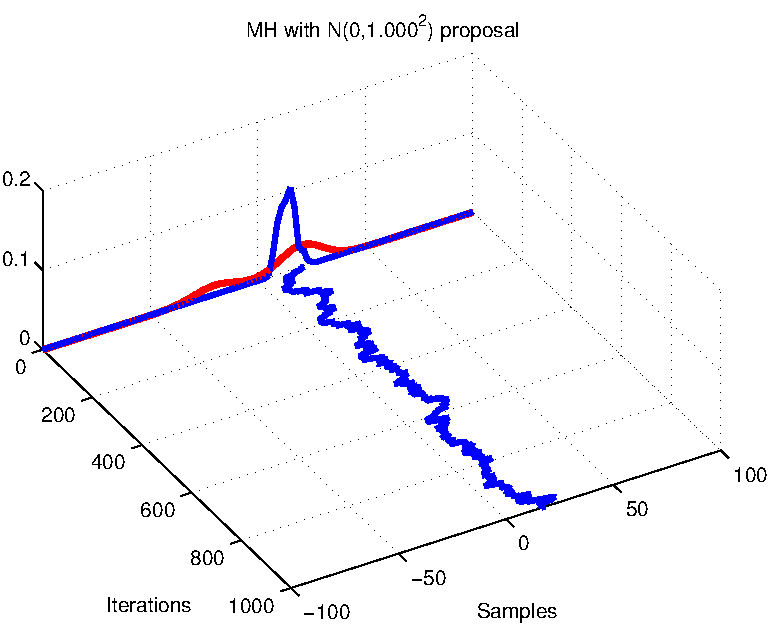
\includegraphics[width=30mm]{mcmcGmmDemoSigma1-3d}}
    \subfigure[]{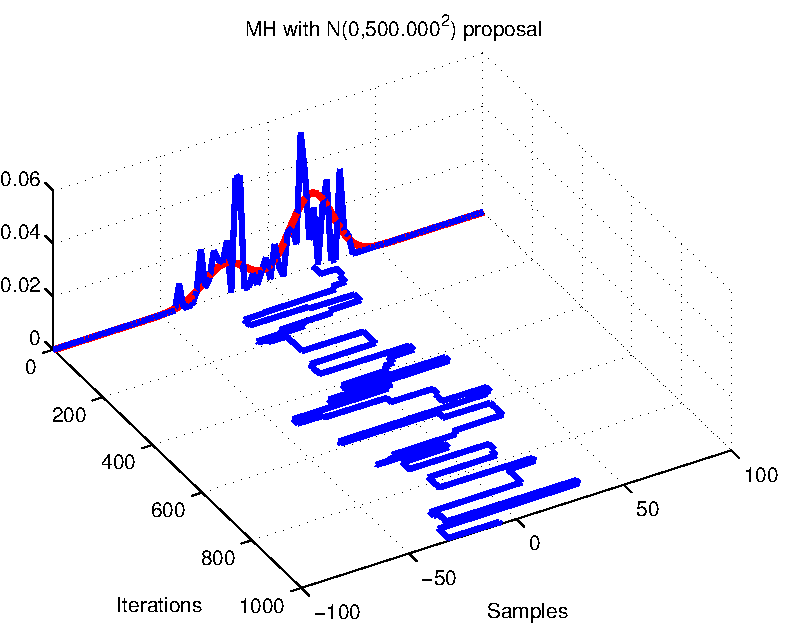
\includegraphics[width=30mm]{mcmcGmmDemoSigma500-3d}}
    \subfigure[]{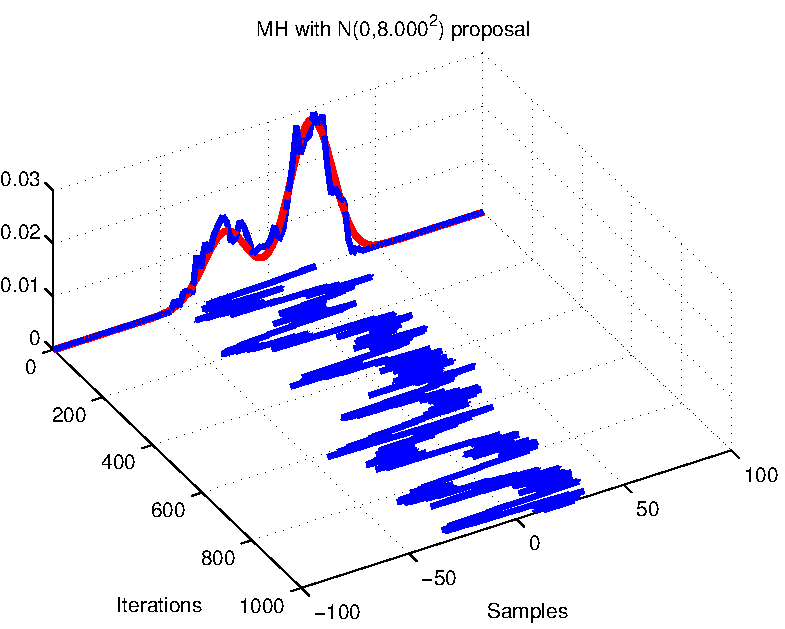
\includegraphics[width=30mm]{mcmcGmmDemoSigma8-3d}}
\end{figure}

\begin{itemize}
    \item When $v = 1$, the chain gets trapped near the starting state and fails to sample from the mode at $\mu = -20$.
    \item When $v = 500$, the chain is very ``sticky", so its effective sample size is low.
    \item Using a variance of $v = 8$ is just right and leads to a good approximation of the true distribution (shown in red).
\end{itemize}
\end{frame}


\begin{frame}{Gibbs sampling is a special case of MH}
\begin{itemize}
    \item Gibbs sampling is a special case of MH.
    \item We move to a new state where $x_i$ is sampled from its full conditional.
    \item But $\bm{x}_{-i}$ is left unchanged.
    \item The acceptance rate of each such proposal
\end{itemize}

\begin{equation*} 
    \alpha = \frac{p(\bm{x}')q(\bm{x}|\bm{x}')}{p(\bm{x})q(\bm{x}'|\bm{x})} = \frac{p(x_i'|\bm{x}_{-i}')p(\bm{x}_{-i}')p(x_i|\bm{x}_{-i}')}{p(x_i|\bm{x}_{-i})p(\bm{x}_{-i})p(x_i'|\bm{x}_{-i})} = 1
\end{equation*} 
\end{frame}

\begin{frame}{Proposal distributions}
\begin{itemize}
    \item A \textbf{valid} proposal $q$ gives a non-zero probability of moving to the states that have non-zero probability in the target.
    \item Example: Gaussian random walk proposal.
    \item For a Gaussian random walk proposal, it is very important to set the variance of the proposal $v$ correctly.
    \begin{itemize}
        \item If the $v$ is too low, the chain will only explore one of the modes.
        \item If the $v$ is too large, most of the moves will be rejected, and the chain will stay in the same state for a long time. 
        \item If we set the proposal's variance just right, the samples clearly explore the support of the target distribution.
    \end{itemize}
    \item \textbf{Optimal acceptance rate:} between 25\% and 40\%.
\end{itemize}
\end{frame}

\section{Speed and accuracy of MCMC}
\begin{frame}{Speed and accuracy of MCMC}
\begin{itemize}
    \item \textbf{Burn-in phase:} Samples collected before the chain has reached its stationary distribution do not come from $p^*$, and are thrown away.
    \item \textbf{Mixing time:} the amount of time a Markov chain takes to converge to the stationary distribution, and forget its initial state.
    \item \textbf{Trace plot:} shows the values the parameter took during the runtime of the chain.
    \item \textbf{Accuracy of MCMC}: samples produced by MCMC are auto-correlated, thus can not be used for estimation.
\end{itemize}
\end{frame}

\section{Auxiliary variable MCMC}    
\begin{frame}{Slice sampling}
\begin{itemize}
    \item Sometimes we can sample by introducing dummy auxiliary variables.
    \item Require require that $\sum_z p(x, z) = p(x)$ and  $p(x, z)$ is easier to sample from than just $p(x)$.
    \item Consider sampling from a univariate, but multimodal, distribution $\tilde{p}(x)$.
    \item Add an auxiliary variable $u$. We define the joint distribution
    \begin{equation*} 
      \hat{p}(x,u)=\begin{cases}
        1/Z_p, & \text{if } 0 \leq u \leq \tilde{p}(x)\\
        0, & \text{otherwise}
      \end{cases}
    \end{equation*} 
    where $Z_p = \int \tilde{p}(x)dx$. 
    \item The marginal distribution over $x$ is given by
    \begin{equation*} 
        \int \hat{p}(x, u)du = \int_0^{\tilde{p}(x)} \frac{1}{Z_p} du = \frac{\tilde{p}(x)}{Z_p}  = p(x)
    \end{equation*} 
\end{itemize}
\end{frame}

\begin{frame}{Slice sampling (cont'd)}
We can sample from $p(x)$ by sampling from $\hat{p}(x, u)$ and then ignoring $u$.  The full conditionals have the form
\begin{equation*} \footnotesize 
    \begin{split}
        p(u|x) & = U_{[0,\tilde{p}(x)]}(u)\\
        p(x|u) & = U_A(x)
    \end{split}
\end{equation*} 
where $A = \{x: \tilde{p}(x)\geq u\}$ it the set of points on or above $u$.

\begin{figure}[h]
\centering
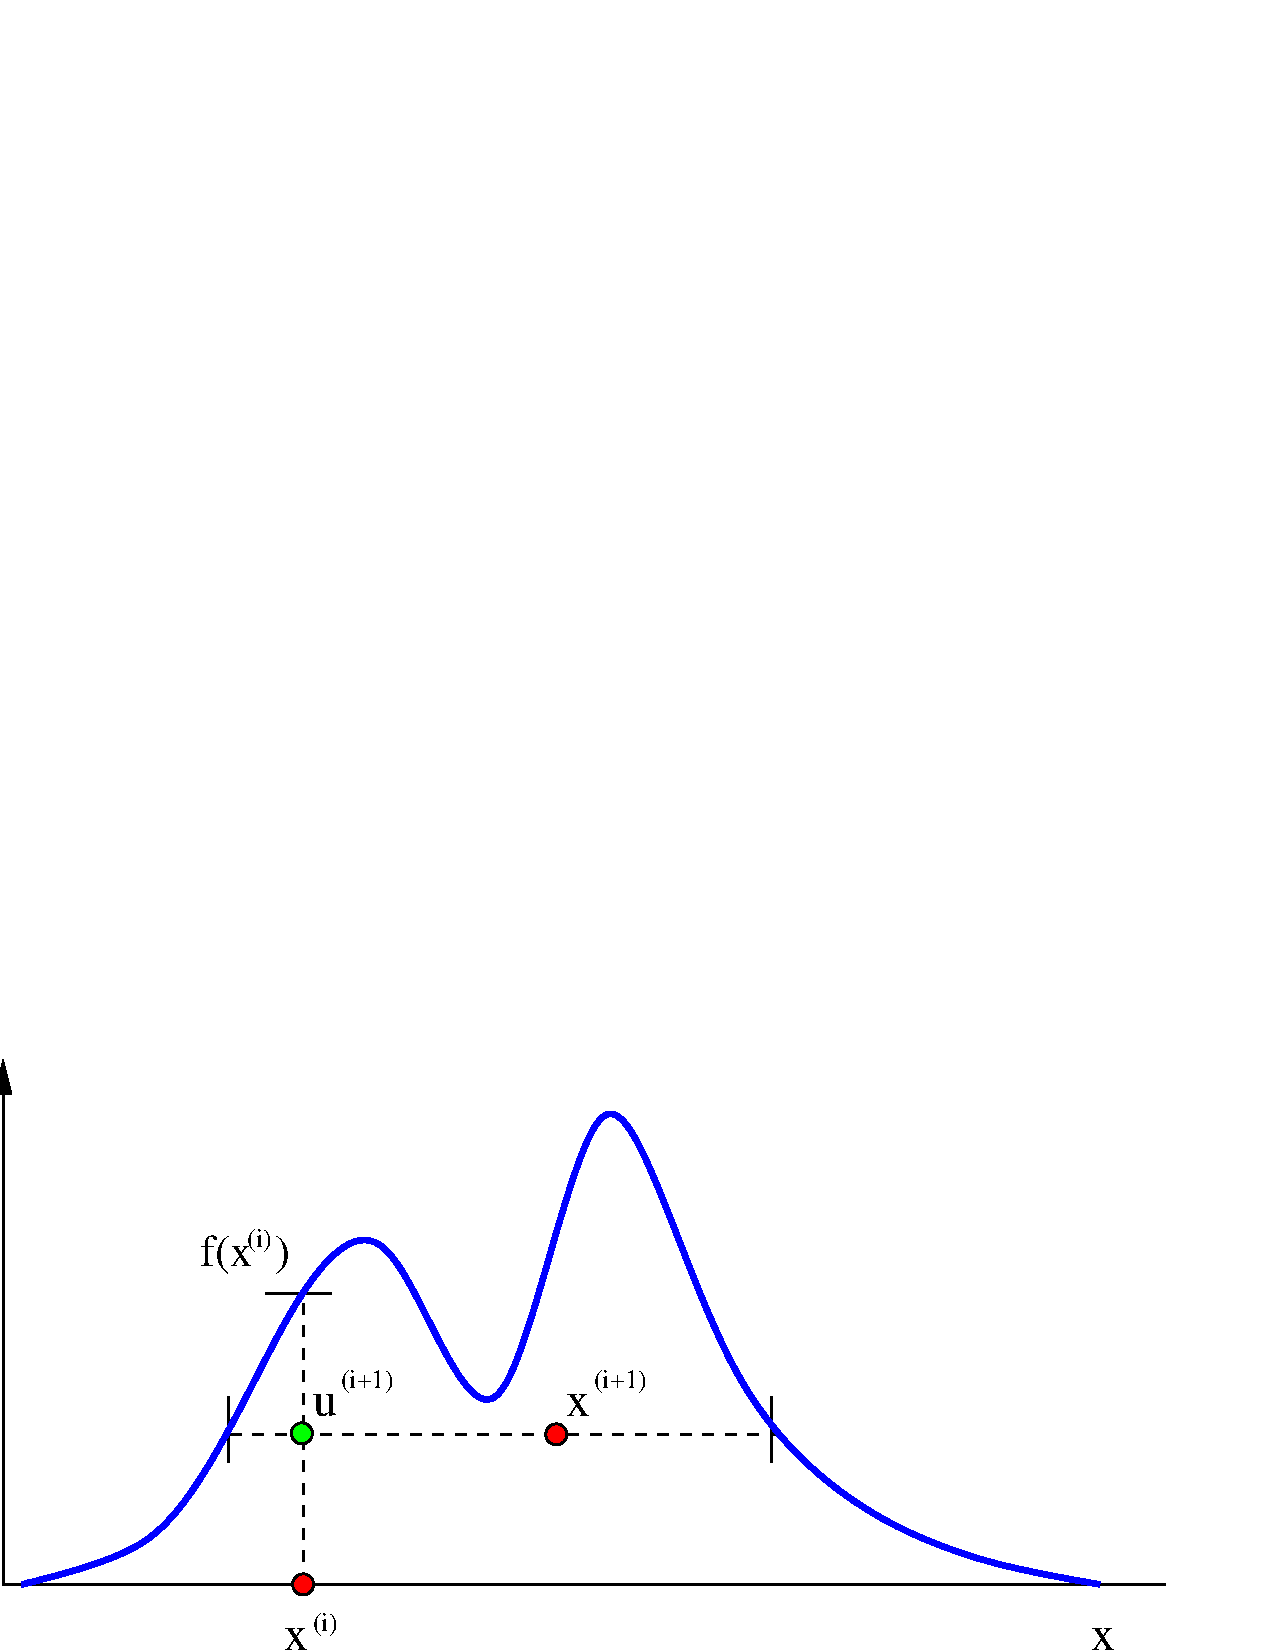
\includegraphics[width=0.5\textwidth]{sliceSampling}
\caption{Illustration of the principle behind slice sampling. Given a previous sample $x^i$ , we sample $u^{i+1}$ uniformly on $[0, f(x^i)]$, which then defines a `slice' through the distribution. We then sample $x^{i+1}$ along the slice where $f(x) \geq u^{i+1}$. Figure generated by \texttt{SliceSamplingDemo1d}.}
\end{figure}
\end{frame}

\end{document}
